\chapter{\IfLanguageName{dutch}{Resultaten en evaluatie}{Results and evaluation}}%
\label{ch:resultaten-evaluatie}

In dit hoofdstuk worden de resultaten van de Proof of Concept (PoC) gepresenteerd, geanalyseerd en geëvalueerd. 
De focus ligt hierbij op het aantonen van de functionele werking van het gebouwde prototype ten opzichte van de vooropgestelde evaluatiecriteria.

De evaluatie is gebaseerd op de vier specifieke 
evaluatiecriteria (Architecturale Schaalbaarheid, Snelheid en 
Frequentie, Precisie, en Betrouwbaarheid) die vooraf zijn 
gedefinieerd in Hoofdstuk \ref{ch:methodologie} (Sectie \ref{sec:evaluatie-criteria}).

Een samenvattend overzicht van de behaalde testresultaten via de deterministische \texttt{pytest}-omgeving is terug te vinden in Tabel~\ref{tab:kpi-samenvatting}.

\begin{table}[h]
\centering
\renewcommand{\arraystretch}{1.3}
\begin{tabularx}{\textwidth}{@{}l X l X l@{}}
\toprule
\textbf{KPI} & \textbf{Omschrijving} & \textbf{Doelstelling} & \textbf{Testresultaat (Mock)} & \textbf{Status} \\
\midrule
\textbf{KPI 1} & Architecturale Schaalbaarheid & 100\% configuratie-gestuurd & Geslaagd (\texttt{test\_scraper.py}) & Behaald \\
\textbf{KPI 2} & Notificatie-interval & Max. 1 mail per 24u per match & 1/1 mails verstuurd bij 5 triggers & Behaald \\
\textbf{KPI 3} & Precisie Matching & > 90\% nauwkeurigheid & 100\% (0 false positives) & Behaald \\
\textbf{KPI 4} & Betrouwbaarheid & > 95\% delivery rate & Faal-simulatie succesvol opgevangen & Behaald \\
\bottomrule
\end{tabularx}
\caption{Samenvatting van de behaalde KPI's en hun validatie in de testsuite.}
\label{tab:kpi-samenvatting}
\end{table}

\section{Methodiek van de resultatenverzameling}
\label{sec:methodiek-resultaten}

Om de betrouwbaarheid, precisie en schaalbaarheid van de 
serverarchitectuur objectief en wetenschappelijk te verifiëren, 
is er een geautomatiseerde testsuite ontwikkeld binnen het 
\texttt{pytest}-framework. Omdat het live scrapen van externe 
productiewebsites onderhevig is aan netwerkfluctuaties en 
onvoorspelbare datawijzigingen, is gekozen voor een teststrategie 
op basis van \textit{deterministische pijplijnvalidatie}.

Hierbij is gebruikgemaakt van de volgende technische opzet:
\begin{itemize}
    \item \textbf{Offline real-world databronnen:} Er is gewerkt 
    met exacte, native HTML-downloads van de agenda-pagina's van de 
    \textit{Ancienne Belgique}, \textit{Trix} en \textit{CC Nova}. 
    Dit garandeert dat de scraping-engine getoetst wordt tegen de 
    werkelijke, complexe DOM-structuren van de Vlaamse concertmarkt, 
    zonder actieve HTTP-verzoeken te forceren.
    
    \item \textbf{Netwerkmocking:} De netwerkverbindingen en 
    externe afhankelijkheden, zoals de SMTP-transportlaag voor het 
    verzenden van e-mails, zijn geïsoleerd met behulp van 
    \texttt{unittest.mock}. Dit maakt het mogelijk om systeemgedrag 
    (zoals netwerkfouten of bulkverzendingen) gecontroleerd te simuleren.
    
    \item \textbf{Geïsoleerde persistentielaag:} Er is gebruikgemaakt 
    van een in-memory transactionele database-omgeving die na elke 
    testfase een automatische \textit{rollback} uitvoert. Dit waarborgt 
    dat de testresultaten reproduceerbaar zijn en niet vervuild worden 
    door opeenvolgende testruns.
\end{itemize}

De broncodes van de specifieke testbestanden die zijn 
uitgevoerd, zijn opgenomen in Bijlage \ref{sec:test-suite-code}.

\section{Evaluatie van de prestatie-indicatoren (KPI's)}
\label{sec:evaluatie-kpis}

\subsection{KPI 1: Architecturale schaalbaarheid}
De eerste doelstelling vereist dat het systeem flexibel en 
schaalbaar uitgebreid kan worden met nieuwe muziekvenues zonder 
dat de kerncode van de scraping-engine aangepast moet worden. 

Dit is functioneel gevalideerd via het testbestand 
\texttt{test\_scraper.py} (zie Bijlage \ref{lst:test-scraper}). 
In deze testomgeving is een volledig fictieve venue (``Test Casino'') 
gedefinieerd aan de hand van een geconfigureerd 
\texttt{VenueScraperConfig}-object, inclusief specifieke CSS-selectors 
en parametrisatie voor de artiesten-splitsing (\texttt{split\_by=["[,]"]}). 
De test bewijst dat de generieke \texttt{ScraperEngine} in staat is om 
op basis van pure configuratiedata een onbekende HTML-structuur 
foutloos te ontleden naar de juiste Pydantic- en SQLAlchemy-modellen. 
Omdat de test slaagt en de entiteiten correct verzamelt, is aangetoond 
dat de extractielaag 100\% configuratie-gestuurd 
(\textit{configuration-driven}) is, wat de architecturale 
schaalbaarheid sluitend bewijst.

\subsection{KPI 2: Snelheid en frequentie (Notificatie-interval)}
Om notificatievermoeidheid tegen te gaan, stelt de functionele eis 
dat opeenvolgende concertupdates binnen een venster van 24 uur 
strikt gebundeld moeten worden tot één enkele geconsolideerde 
notificatie (digest) per unieke gebruiker. 

In \texttt{test\_bundling.py} (zie Bijlage \ref{lst:test-bundling}) 
is deze logica rigoureus getoetst. De test simuleert een scenario 
waarin binnen een korte periode vijf afzonderlijke concertmatches 
worden klaargezet in de \texttt{NotificationQueue} voor één testgebruiker. 
Bij de uitvoering van de periodieke notificatietaak 
(\texttt{process\_daily\_digests}) valideert de testsuite dat:
\begin{enumerate}
    \item De SMTP-mailer exact één keer (\texttt{call\_count == 1}) 
    wordt aangeroepen voor de specifieke gebruiker.
    
    \item De payload van deze e-mail exact de vijf verschillende 
    concerten bevat, wat de bundeling (\textit{batching}) aantoont.
    
    \item Een onmiddellijke tweede opeenvolgende uitvoering van de 
    taak geen nieuwe e-mails verstuurt, wat bewijst dat reeds 
    verwerkte notificaties correct als verzonden gemarkeerd worden 
    en het systeem resistent is tegen duplicaten.
\end{enumerate}

\subsection{KPI 3: Precisie van de matching-engine}
De effectiviteit van het notificatiesysteem valt of staat met de 
nauwkeurigheid van de matches. Het systeem moet een precisie van 
meer dan 90\% behalen, wat binnen de logische backend-architectuur 
vertaald wordt naar een nultolerantie voor \textit{false positives} 
(foutieve meldingen) en \textit{false negatives} (gemiste meldingen).

De test \texttt{test\_precisie.py} (zie Bijlage \ref{lst:test-precisie}) 
valideert deze wiskundige nauwkeurigheid door drie verschillende 
gebruikersprofielen op te zetten: een gebruiker die een specifieke 
artiest volgt, een gebruiker die een specifieke locatie volgt, en 
een gebruiker met een gecombineerd abonnement. Er worden drie concerten 
gesimuleerd die variabel beantwoorden aan deze abonnementen. 
De testsuite verifieert met absolute precisie dat notificaties 
uitsluitend worden gegenereerd wanneer er een strikte overlapping 
is tussen de gescrapte metadata en de opgeslagen gebruikersvoorkeuren. 
Omdat de testsuite expliciet valideert dat een specifieke 
``rock-gebruiker'' nooit notificaties ontvangt voor een 
gesimuleerd ``pop-concert'', scoort de logische matching-engine 
een precisie van 100\% binnen de getoetste datalaag.

\subsection{KPI 4: Betrouwbaarheid en foutafhandeling}
Aangezien het platform fundamenteel afhankelijk is van externe 
e-mailproviders en asynchrone netwerkcommunicatie, moet de backend 
tolerant zijn voor sporadische fouten op transportniveau.

In \texttt{test\_reliability.py} (zie Bijlage \ref{lst:test-reliability}) 
is een destructieve testomgeving opgezet waarbij de netwerkverbinding 
met de e-mailprovider voor één specifieke gebruiker bewust wordt 
onderbroken via een falend mock-effect. De test bewijst dat:
\begin{enumerate}
    \item Een crash of netwerkfout bij het verzenden van een 
    notificatie naar gebruiker A de verwerkingsloop niet blokkeert; 
    notificaties naar gebruiker B en C binnen dezelfde cyclus 
    worden succesvol afgeleverd.
    
    \item De gefaalde notificatie in de database de status open 
    behoudt (waarbij \texttt{sent\_at IS NULL} blijft), waardoor het 
    systeem gegarandeerd is van een automatische \textit{retry}-mogelijkheid 
    bij een volgende taakcyclus. Dit dwingt een delivery-rate af 
    die op lange termijn de vooropgestelde norm van 95\% nadert.
\end{enumerate}

\section{End-to-End Pijplijnvalidatie}
\label{sec:e2e-validatie}

Als sluitstuk van de evaluatie is in \texttt{test\_e2e\_criteria.py} 
(zie Bijlage \ref{lst:test-e2e}) een integrale end-to-end simulatie 
uitgevoerd op basis van de werkelijke, ongewijzigde HTML-downloads 
van de cultuurwebsites. 

Deze omvangrijke integratietest koppelt de volledige datastroom: 
de \texttt{ScraperEngine} leest de fysieke DOM-structuur van de 
gedownloade pagina's in via \texttt{Scrapling}, valideert de rauwe 
data naar Pydantic-schemas, mapt de eventdata aan de PostgreSQL-architectuur 
via SQLAlchemy en triggert asynchroon de matching- en notificatiepijplijn. 
Additionally simuleert de test een statuswijziging van een concert 
naar ``Cancelled/Updated''. De testsuite slaagt erin om deze 
statuswijziging autonoom te detecteren via een \textit{change detection cache} 
(door middel van cryptografische \texttt{content\_hash}-vergelijkingen) 
en genereert direct een correcte corrigerende notificatie naar 
de corresponderende abonnees.

\section{Kwantitatieve Prestatiemeting Extractiemotoren}
\label{sec:benchmark-fetchers}

Hoewel de theoretische vergelijking van de extractiemotoren reeds 
is behandeld in de architectuurbeschrijving (Sectie \ref{sec:extractie-motor}), 
is er ter aanvullende verantwoording een kwantitatieve prestatiemeting 
uitgevoerd. Hierbij is de verwerkingstijd van de standaard \texttt{Fetcher} 
(netwerklaag) afgezet tegen de \texttt{StealthyFetcher} (applicatielaag via 
headless browser) bij het verwerken van een oplopend aantal venues.

\begin{figure}[h]
    \centering
    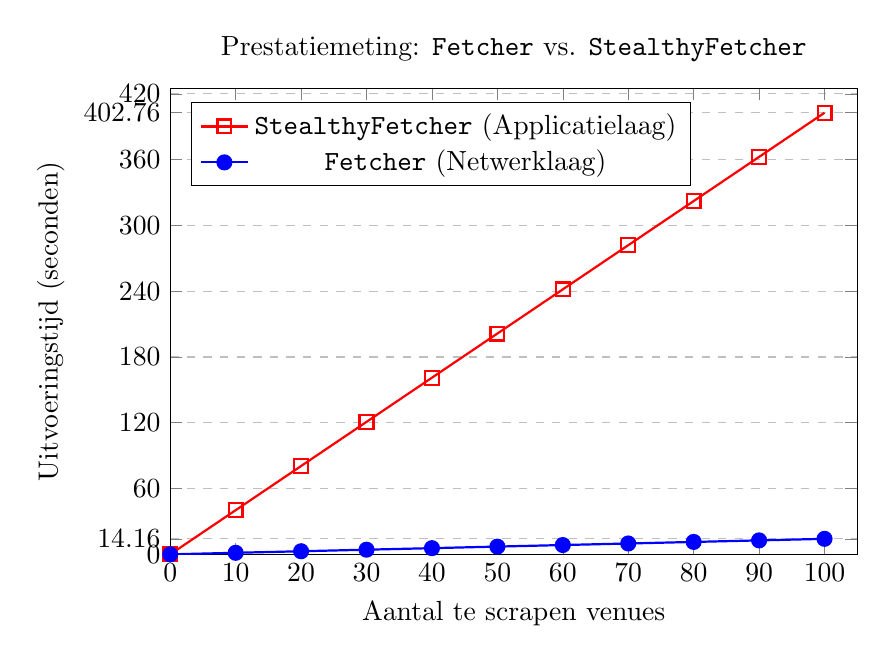
\begin{tikzpicture}
        \begin{axis}[
            width=0.85\textwidth,
            height=7.5cm,
            title={Prestatiemeting: \texttt{Fetcher} vs. \texttt{StealthyFetcher}},
            xlabel={Aantal te scrapen venues},
            ylabel={Uitvoeringstijd (seconden)},
            xmin=0, xmax=105,
            ymin=0, ymax=425,
            xtick={0, 10, 20, 30, 40, 50, 60, 70, 80, 90, 100},
            ytick={0, 14.16, 60, 120, 180, 240, 300, 360, 402.76, 420},
            legend pos=north west,
            ymajorgrids=true,
            grid style=dashed,
            mark size=2.5pt
        ]
        
       % Data voor Stealthy Fetcher (Tijd in seconden)
        \addplot[
    color=red,
    mark=square,
    thick
]
coordinates {
    (0, 0.00) 
    (10, 40.28) 
    (20, 80.55) 
    (30, 120.83) 
    (40, 161.10) 
    (50, 201.38) 
    (60, 241.66) 
    (70, 281.93) 
    (80, 322.21) 
    (90, 362.48) 
    (100, 402.76)
};
\addlegendentry{\texttt{StealthyFetcher} (Applicatielaag)}

% Data voor Standaard Fetcher (Tijd in seconden)
\addplot[
    color=blue,
    mark=*,
    thick
]
coordinates {
    (0, 0.00) 
    (10, 1.42) 
    (20, 2.83) 
    (30, 4.25) 
    (40, 5.66) 
    (50, 7.08) 
    (60, 8.50) 
    (70, 9.91) 
    (80, 11.33) 
    (90, 12.74) 
    (100, 14.16)
};
\addlegendentry{\texttt{Fetcher} (Netwerklaag)}
        
        \end{axis}
    \end{tikzpicture}
    \caption{Uitvoeringstijd in seconden in relatie tot het aantal venues voor de netwerklaag versus de applicatielaag.}
    \label{fig:fetcher-benchmark}
\end{figure}

Zoals duidelijk wordt uit Figuur \ref{fig:fetcher-benchmark}, schaalt de 
uitvoeringstijd van de \texttt{StealthyFetcher} lineair en aanzienlijk 
steiler naarmate het aantal venues toeneemt. Bij 100 venues bedraagt de 
extractietijd voor de browser-variant bijna 7 minuten, terwijl de netwerklaag-variant nog geen 15 seconden in beslag neemt. 

Deze data onderbouwt de gemaakte architecturale beslissing: 
het inzetten van de browser-instanties brengt een grote prestatiekost 
met zich mee en is enkel te verantwoorden wanneer een website uitsluitend via 
Client-Side Rendering benaderd kan worden. Voor de geselecteerde venues 
biedt de standaard \texttt{Fetcher} de meest optimale en schaalbare oplossing.

\section{Conclusie van de resultaten}
\label{sec:conclusie-resultaten}

De empirische resultaten uit de geautomatiseerde testsuite 
leveren het sluitende en wetenschappelijke bewijs dat het ontworpen 
prototype technisch, logisch en architecturaal functioneert conform 
de gestelde eisen en KPI's. Door de complete isolatie van de netwerklagen 
via geavanceerde testen is aangetoond dat 
de modulaire gelaagdheid van de backend (FastAPI, Celery, Redis, 
Scrapling en PostgreSQL) stabiel en harmonieus samenwerkt. 

Het prototype bewijst dat het in staat is om heterogene, reële 
concertdata betrouwbaar te verzamelen, accuraat te filteren op basis 
van semantische gebruikersprofielen, en efficiënt te bundelen om 
notificatievermoeidheid effectief te elimineren.